\section{Selection Process} \label{Sec_selectionp}

Since the main aim of the project is to improve the positioning system of the existing setup, several  other techniques were discussed, ending up in four methods namely ``\textit{triangulation}'',``\textit{pattern recognition}'',``\textit{radio frequency identification}'', ``\textit{map-based localization}''. The pros and cons were listed and the mentioned techniques were compared. The following section deals with a brief description of the above mentioned techniques.\\

\subsection{Triangulation} %stefan
Since the plant has a specified size in which the location of multiple objects has to be performed the method of triangulation is one promising technic in which research was made. 
Triangulation was already a common principle of measurement in the 18th century and it is divided into active and passive triangulation. Passive triangulation is a geometrical method based on two measurement stations which positions are known exactly. At these two measurement points angels of the desired point in space are measured to compute the localization in the specified coordinate system (x, y, z) with trigonometrical formulas.
With respect to the system setup used in the 18th century nowadays two cameras are installed to perform a geographical method of 3D object-data estimation as shown in fig. \ref{Triangulation} \cite{Prinzip3DVideometrie.}.
\begin{figure}[!htbp]
\centering
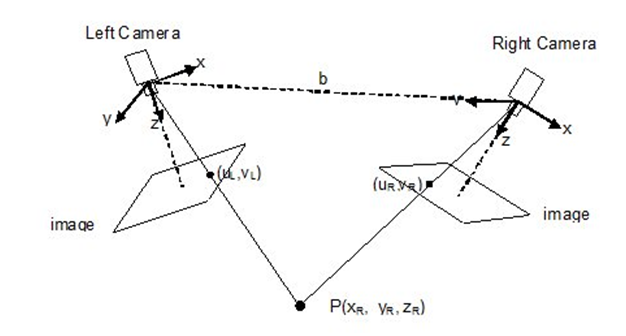
\includegraphics[width = 16cm]{Pictures/Triangulation}
\caption{Passive triangulation setup with two cameras [3]}
\label{Triangulation}
\end{figure}\\
To solve the problem of position estimation, it is necessary to know the parameters of the left and the right camera visualized in the figure. In theory the triangulation is trivial, since each and every point of the images of the respective cameras maps to a line in 3D space. If a pair of corresponding points, in the case of the pipesless plant it would be an AGV is found, the projection of a point x in 3D space can be computed. 
Active triangulation in comparison to passive triangulation needs one camera and at least one source of structured light (e.g. Laser). The geometrical location and orientation of the camera and light source in space need to be known. Two possible setups with either a laser point or a stripe as structured light are shown in fig. \ref{ative_Triangulation} \cite{MultiObjectTriangulation.}.
\begin{figure}[!htbp]
\centering
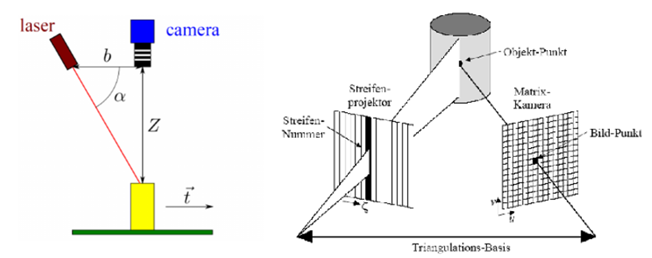
\includegraphics[width = 16cm]{Pictures/acticetriangulation}
\caption{Active triangulation [3]}
\label{ative_Triangulation}
\end{figure}\\
To solve the active triangulation problem, the structured light has to point an object which location is desired to estimate. If this point is found on the 2D image of the camera, a triangulation with basic trigonometrical formulas which are using the properties and parameters of the camera and light source can be performed and the position of the AGV can be estimated. 
\pagebreak
\subsubsection*{Implementation} 
One possible way to implement a solution for the passive triangulation is to attach 2 high resolution cameras with USB 3.0 on two edges of the plant as shown in fig. \ref{ativeTriangulationimplementation}.\\
\begin{figure}[!htbp]
	\centering
	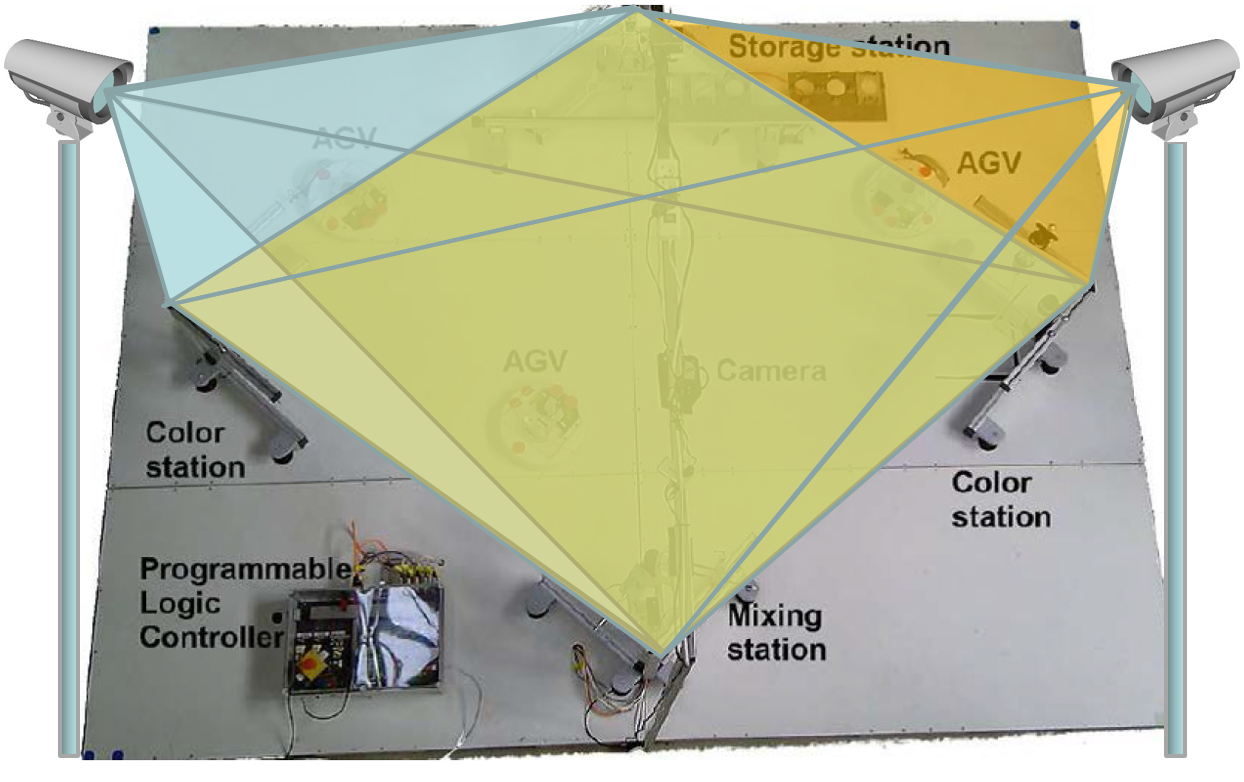
\includegraphics[width = 16cm]{Pictures/triangulationimplementatio}
	\caption{Implementation of passive triangulation}
	\label{ativeTriangulationimplementation}
\end{figure}\\%
The left and right camera are sequentially taking pictures which are transmitted to the plants computer where the image processing takes place.\\ 
\pagebreak
Based on the research made , two tables with advantages and disadvantages of the two triangulation systems are created.
\begin{table}[!htbp]
\centering
\begin{tabular}{|l|l|}
\hline
\multicolumn{2}{|c|}{\textbf{Passive Triangulation}}                                                                                                                  \\ \hline
\multicolumn{1}{|c|}{\textbf{Pro}}                                                                                    & \multicolumn{1}{c|}{\textbf{Con}}   \\ \hline
Upgrade to USB 3.0 for faster data transmitting possible                                                                   & Light dependent                          \\ \hline
\begin{tabular}[c]{@{}l@{}}Upgrade to a camera with higher resolution to reduce \\ measurement error possible\end{tabular} & New concept of orientation may be needed \\ \hline
No Fish-Eye-Lense problem                                                                                                  & Limited range of observation             \\ \hline
Low cost                                                                                                                   &                                          \\ \hline
\end{tabular}
\caption{Pros and cons points of passive triangulation}
\label{pro_con_passive_tri}
\end{table}
\begin{table}[!htbp]
\centering
\begin{tabular}{|l|l|}
\hline
\multicolumn{2}{|c|}{\textbf{Active Triangulation}}                                                                                                                     \\ \hline
\multicolumn{1}{|c|}{\textbf{Pro}}                                                                                    & \multicolumn{1}{c|}{\textbf{Con}}     \\ \hline
Upgrade to USB 3.0 for faster data transmitting possible                                                                   & New unknown laser technology is needed     \\ \hline
\begin{tabular}[c]{@{}l@{}}Upgrade to a camera with higher resolution to reduce \\ measurement error possible\end{tabular} & High costs for several lasers (one per AGV) \\ \hline
Easy detection of laser points on camera image                                                                             & Laser needs to move while AGVs are moving  \\ \hline
                                                                                                                           & Limited range of observation               \\ \hline
                                                                                                                           & Light dependent                            \\ \hline
\end{tabular}
\caption{Pros and cons points of active triangulation}
\label{pro_con_active_tri}
\end{table}
\pagebreak
\subsection{Pattern Recognition} %medhini
\subsubsection*{Summary}
In this type of localization, estimation of the robot is done in indoor environments using
only on-board sensors, namely a web-cam and a compass. The ceiling of the plant is constructed with a pattern of static landmarks whose positions are known a priori. All landmarks are indistinguishable against each other and might additionally be distributed along the ceiling in a periodic pattern. The landmark attached to the ceiling can be lights, QR codes, sensors or other
reference points. The ceiling is used, since it is immune to changes. A camera is installed on the robot, which takes snapshots of the ceiling. The robot pose relative to the landmark is  calculated with the help of the distance of the landmark to the center of the image and its angle relatively to the direction of the  robot motion. An IMU device is additionally used to give the absolute orientation of the robot in the plant. The Markov Localization (ML) algorithm is used to estimate
the belief grid of the robot position inside the environment. 

\begin{figure}[!htbp]
	\centering
	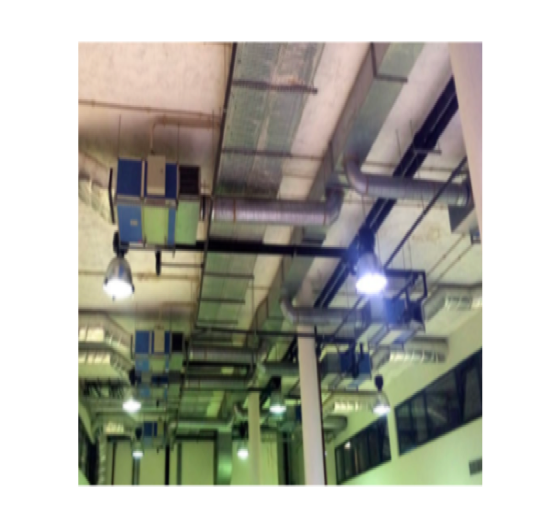
\includegraphics[width = 10cm]{Pictures/PR.png}
	\caption{Ceiling with periodic patterns of lamps acting as landmarks. }
	\label{Pattern Recognition}
\end{figure}
\subsubsection*{Implementation}
The goal is to compute the pose of a mobile robot inside an indoor environment using a camera and an IMU device. As mentioned, Markov Localization is used to create a belief grid of the robot in the plant environment. This is done with the help of the snapshots of the ceiling taken by the camera. As seen in the figure \ref{PatternRecognition1}, the blue and black areas have lower belief and green and yellow areas have higher belief. The obtained pattern is evaluated and based on the pattern, the position of the robot is estimated. Thus with the help of the camera and the IMU device, both the position and orientation is obtained. 


\begin{figure}[!htbp]
	\centering
	\begin{minipage}{.5\textwidth}
		\centering
		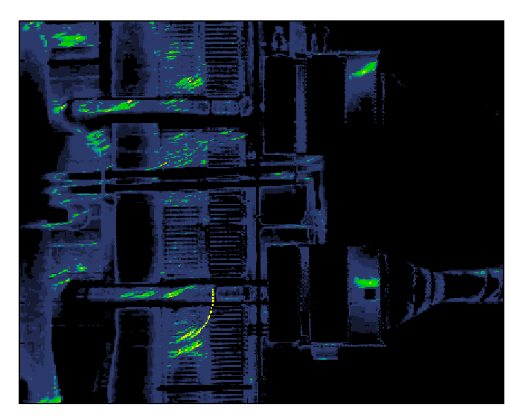
\includegraphics[width = 7cm]{Pictures/beliefgrid.png}
		\caption{Belief grid of the robot in the plant}
		\label{PatternRecognition1}
	\end{minipage}%
	\begin{minipage}{.5\textwidth}
		\centering
		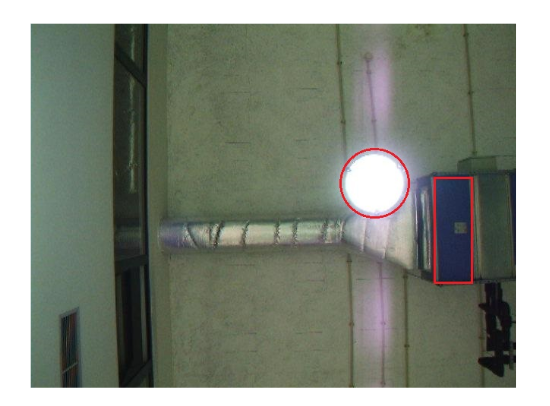
\includegraphics[width = 8cm]{Pictures/snapshot.png}
		\caption{Snapshot of the ceiling }
		\label{PatternRecognition2}
	\end{minipage}
\end{figure}

\subsubsection*{Pro and con}
Based on the research,the advantages and disadvantages of Mobile Robot Localization based on Pattern Recognition are created.
\begin{table}[!htbp]
	\centering
	\begin{tabular}{|l|l|}
		\hline
		
		\multicolumn{1}{|c|}{\textbf{Pro}}                                                                                    & \multicolumn{1}{c|}{\textbf{Con}}   \\ \hline
		\begin{tabular}[c]{@{}l@{}}The ceiling is usually immune to changes                                                                  
			as a  \\ reference and implement  landmarks
			on the ceiling itself  \end{tabular}                                                & \begin{tabular}[c]{@{}l@{}}Complex and many changes have to be \\ added to the plant   \end{tabular}                                    \\ \hline
		
		
		No Fish-Eye-Lense problem                                                                                            & Cost intensive                                 \\ \hline
		& Light dependent                            \\ \hline
		
	\end{tabular}
	\caption{Pros and cons points of Mobile Robot Localization based on Pattern Recognition
	}
	\label{pro_con_Mobile Robot Localization based on Pattern Recognition
	}
\end{table}
\pagebreak

\subsection[RFID]{RFID\footnote{Stephan}} % stephan around 2 pages
\subsubsection*{Summary} 
One of the possible solutions to solve the challenging problem of indoor localization is the use of the Radio-frequency Identification (RFID) technology. The main areas of this technology is indeed still supply chains, transport, manufacturing, personnel access, animal tagging, toll collection \cite{Bai_overviewof},  but also has become popular in localizing objects and persons. Where in the main applications only the identification has to be realized, also the strength of the signals is important to estimate the position of a certain object.\\
The main idea of those systems is that a reader detects a tag and reads its information. The technology can be divided into three main types: passive, semi-passive and active systems. A passive system, like it is been shown in fig. \ref{RFID_Passive}, consists of a reader, which is connected to an antenna and a computer and a passive tag.\\
\begin{figure}[!htbp]
\centering
\begin{minipage}{.5\textwidth}
\centering
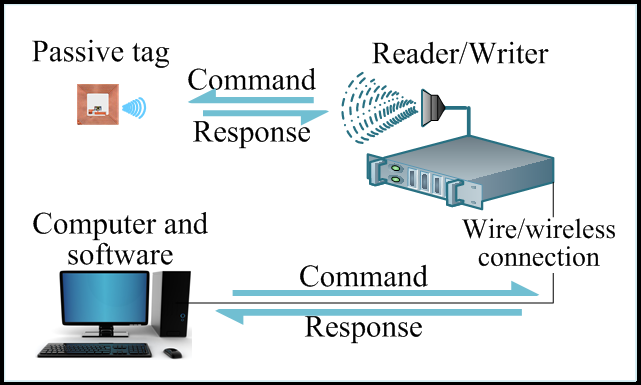
\includegraphics[width = 7cm]{Pictures/RFID_Passive}%
\caption{Passive RFID System}
\label{RFID_Passive}
\end{minipage}%
\begin{minipage}{.5\textwidth}
\centering
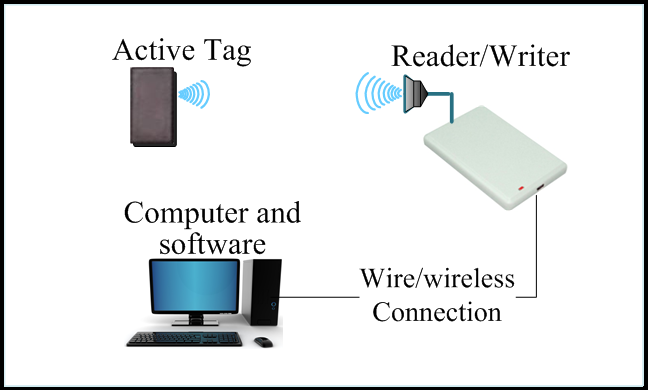
\includegraphics[width = 7cm]{Pictures/RFID_Active}%
\caption{Active RFID System}
\label{RFID_Active}
\end{minipage}
\end{figure}\\
The system is called passive, because the power supply is realized by the radio signal of the reader. In case where the tag is in the reading range of the reader, the tags gets enough power to send predefined information (for example ID) back. The active system (see fig.\ref{RFID_Active}) in comparison has an active tag which has an own power supply. The semi-passive tag has a battery build in that the tag has more power to communicate, but is not used to generate radio frequency signals.\\ 
Another classification of RFID systems is the frequency of the radio waves. It can reach from 0.135 MHz (Low Frequency) to 5875 MHz (Super High Frequency). The table \ref{RFID_Systems} gives an overview about the systems related to reading ranges, reading rates and the ability to read near metal or water.\\
\begin{table}[!htbp]
\centering
\begin{tabular}{c}
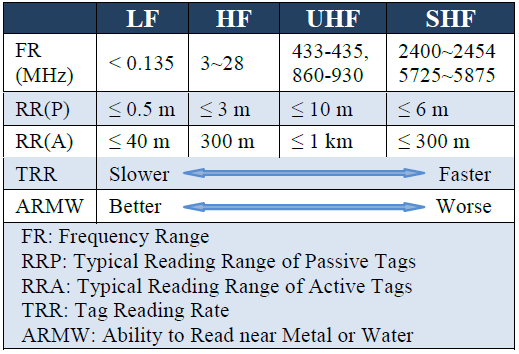
\includegraphics[width = 9cm]{Pictures/RFID_Systems}
\end{tabular}
\caption{Overview RFID systems}
\label{RFID_Systems}
\end{table}\\
It can be seen that the passive systems in general have a smaller reading range then the active systems and has a bigger data rate. But it has also to be take into account, that passive tags are cheaper then active tags.   
\subsubsection*{Implementation}
There are mainly two different ways to realize a localization system of the AGVs in the pipeless plant. Based on the fact that the plant has a size of 3 by 4 meter, the tracking can be carried out with a passive system in which a couple of passive tags on the floor can be used as landmarks. In this case the reader plus the antenna would be placed on the AGV and localize with the help of the detected tags. The other systems consists of three or four reader in each corner of the plant and an active tag on each AGV.
\pagebreak
\subsubsection*{Pro and con}
Based on the research made, two tables with advantages and disadvantages of the two RFID systems are created.\\ 
\begin{table}[!htbp]
\centering
\begin{tabular}{|l|l|}
\hline
\multicolumn{2}{|c|}{\textbf{Active RFID system}}                                                                                                                                                                                \\ \hline
\multicolumn{1}{|c|}{\textbf{Pro}}                                                                                & \multicolumn{1}{c|}{\textbf{Con}}                                                                            \\ \hline
Light independent                                                                                                 & Prototype more expansive (3 reader + avtive tags)                                                            \\ \hline
Space unlimited                                                                                                   & \begin{tabular}[c]{@{}l@{}}Datarate is related to the amount of\\ detected tags a the same time\end{tabular} \\ \hline
\begin{tabular}[c]{@{}l@{}}Localization only has to be realized in\\ a bigger area - medium accuracy\end{tabular} & \begin{tabular}[c]{@{}l@{}}Anticollision need, cause more AGVs are\\ used at the same time\end{tabular}      \\ \hline
\begin{tabular}[c]{@{}l@{}}Wired communication between reader and \\ computer possible\end{tabular}               & \begin{tabular}[c]{@{}l@{}}Signal strength can be influenced by envirnonment\\ (metal or water)\end{tabular} \\ \hline
Simple algorithm (Trilateration)                                                                                  &                                                                                                              \\ \hline
\end{tabular}
\caption{Pro and cons of active RFID system}
\label{my-label}
\end{table}
\begin{table}[!htbp]
\centering
\begin{tabular}{|l|l|}
\hline
\multicolumn{2}{|c|}{\textbf{Passive RFID system}}                                                                                                                                                                                            \\ \hline
\multicolumn{1}{|c|}{\textbf{Pro}}                                                                                             & \multicolumn{1}{c|}{\textbf{Con}}                                                                            \\ \hline
Light independent                                                                                                               & \begin{tabular}[c]{@{}l@{}}Communication between AGV and computer \\ has to be realized\end{tabular}         \\ \hline
Space unlimited                                                                                                                & \begin{tabular}[c]{@{}l@{}}Data rate is related to the amount of\\ detected tags a the same time\end{tabular} \\ \hline
\begin{tabular}[c]{@{}l@{}}Localization only has to be realized between\\ four tags (small area) - high accuracy\end{tabular} & \begin{tabular}[c]{@{}l@{}}Anticollision need, cause more tags are\\ detected at the same time\end{tabular}  \\ \hline
Simple algorithm (Trilateration)                                                                                               &                                                                                                              \\ \hline
Prototype cheap (1 reader + passive tags)                                                                                      &                                                                                                              \\ \hline
\end{tabular}
\caption{Pro and cons passive RFID system}
\label{Pro and Cons of the passive RFID system}
\end{table}
\pagebreak
\subsection{Map-Based Localization\cite{mbl}} %abdul
\subsubsection*{Summary}
AMCL (Adaptive Monte Carlo Localization) is a probabilistic localization system for a robot moving in 2D. It implements the adaptive (or KLD-sampling) Monte Carlo localization\cite{acml1}\cite{acml2} approach, which uses a particle filter to track the pose of a robot against a known map.
\begin{figure}[!htbp]
	\centering
	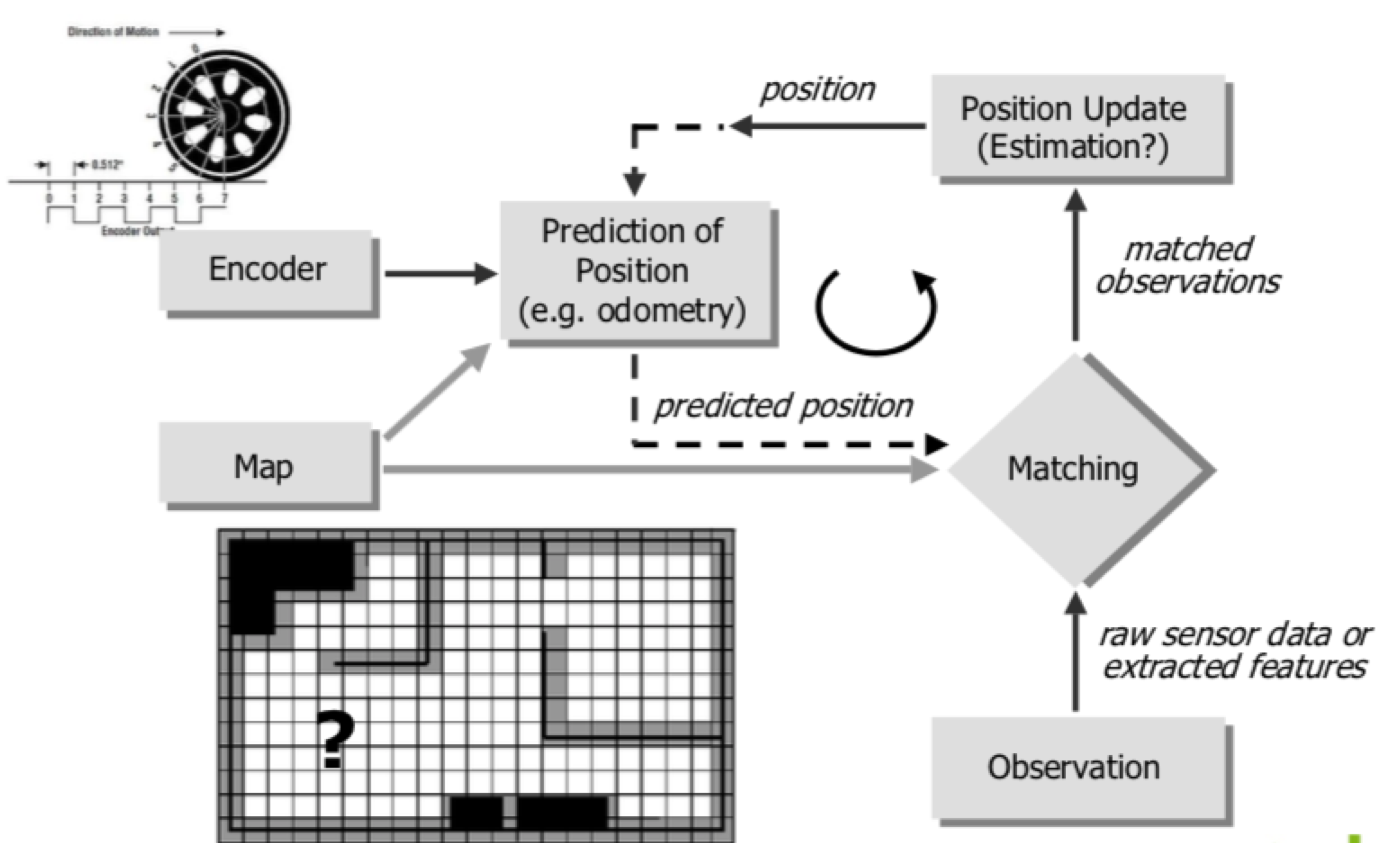
\includegraphics[width = 15cm]{Pictures/amcl}
	\caption{Adaptive Monte Carlo localization}
	\label{amcl}
\end{figure}\\
amcl takes in a laser-based map, laser scans, and Odom scan, and outputs pose estimates (see fig.\ref{amcl}). On startup, amcl initializes its particle filter according to the parameters provided. Note that, because of the defaults, if no parameters are set, the initial filter state will be a moderately sized particle cloud centered about (0,0,0).
\\
\subsubsection*{Implementation}
To implement such a technique a global and local map should be created as shown in fig. \ref{global_map} and fig. \ref{local_map}.
\begin{figure}[!htbp]
	\centering
	\begin{minipage}{.5\textwidth}
		\centering
		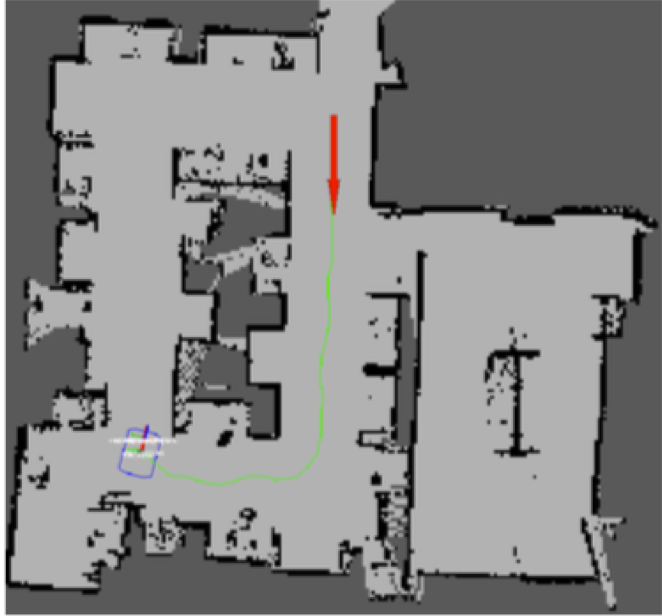
\includegraphics[width = 6cm]{Pictures/global}%
		\caption{Global Map}
		\label{global_map}
	\end{minipage}%
	\begin{minipage}{.5\textwidth}
		\centering
		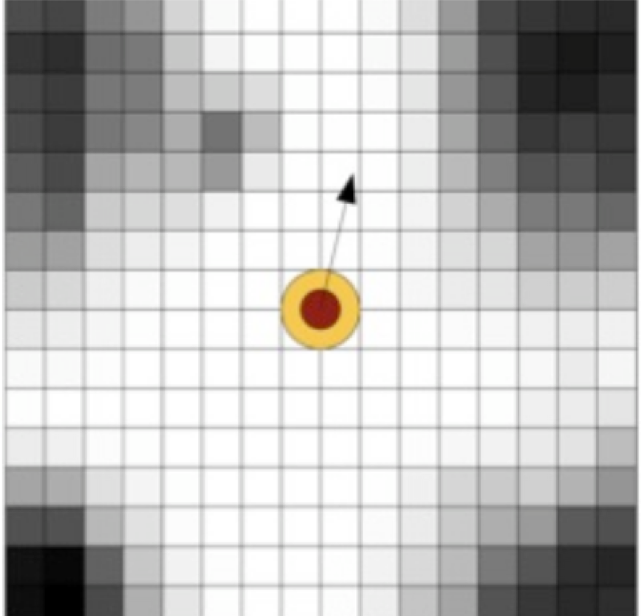
\includegraphics[width = 6cm]{Pictures/local}%
		\caption{Local Map}
		\label{local_map}
	\end{minipage}
\end{figure}
\begin{itemize}
\item SLAM (Simultaneous Localization and Mapping) is a technique used in mobile robotics in which a robot builds a map of an unknown environment, keeping at the same time track of its localization in this environment.\\
\end{itemize}
\begin{itemize}
\item Adaptive Monte Carlo Localization
\\
Given a map of the environment, the goal of the algorithm is for the robot to determine its pose within the environment.
\\
At every time \(t\) the algorithm takes as input the previous belief \(X_{t-1}=\big\{x_{t-1}^1, x_{t-1}^2, ...., x_{t-1}^M\big\} \),  an actuation command \(u_t\), and data received from sensors \(z_t\); and the algorithm outputs the new belief \(X_t\).
\end{itemize}
\begin{itemize}
	\item Orientation Correction
	\begin{figure}[!htbp]
		\centering
		\begin{minipage}{.5\textwidth}
			\centering
			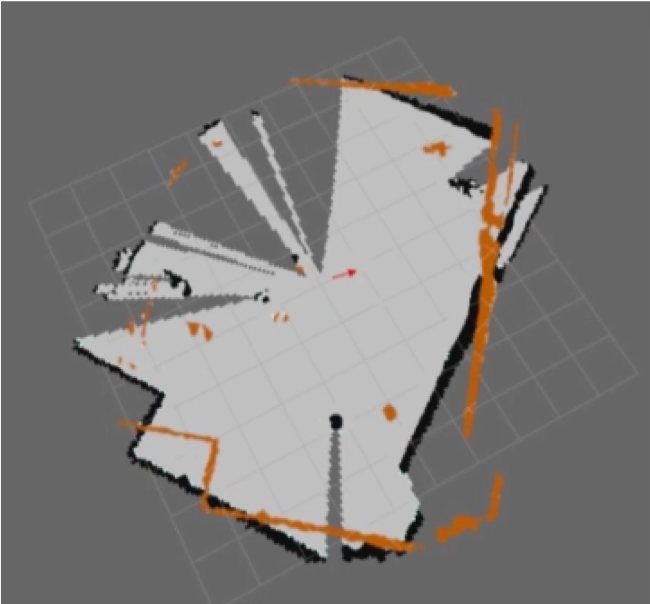
\includegraphics[width = 6cm]{Pictures/robotorientation}%
			\caption{Robot Orientation}
			\label{robot_orientation}
		\end{minipage}%
		\begin{minipage}{.5\textwidth}
			\centering
			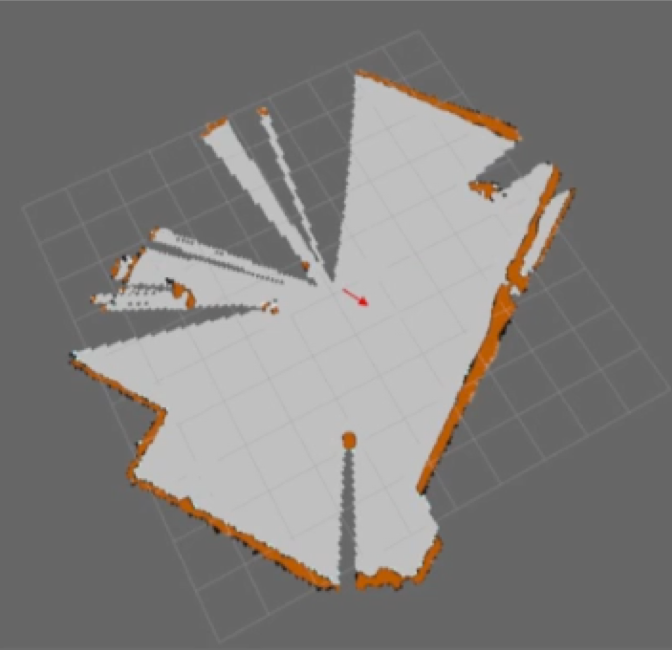
\includegraphics[width = 6cm]{Pictures/correctionwithglobalmap}%
			\caption{Correction with global map}
			\label{correction_with_globalmap}
		\end{minipage}
	\end{figure}\\
 	Initially the robot assumes a position as shown in fig.\ref{robot_orientation}, and as it moves it begins to re-correct it's estimated orientation using the static obstacle with the global map as a reference as shown in fig. \ref{correction_with_globalmap}. 
\end{itemize}
\subsubsection*{Pro and con}
Based on the research made, two tables with advantages and disadvantages of the two Map-Based Localization systems are created.\\ 
\begin{table}[!htbp]
	\centering
	\begin{tabular}{|l|l|}
		\hline
		\multicolumn{2}{|c|}{\textbf{Using Ultrasonic Sensor}}                                                                                                                                                                                \\ \hline
		\multicolumn{1}{|c|}{\textbf{Pro}}                                                                                & \multicolumn{1}{c|}{\textbf{Con}}                                                                            \\ \hline
		Cheap \euro3/each                                                                                                & Scan angle 30\degree                                                            \\ \hline
		Easy hardware Installation                                                                                                   & Similar landmarks cause localization error 
		\\ \hline
		\begin{tabular}[c]{@{}l@{}}Faster feedback than the previous camera\\ based localization system\end{tabular}
		& High computational effort for large plant     
		\\ \hline
		Scan range 4.5 meters
		& \begin{tabular}[c]{@{}l@{}}Robots should start at every launch from static\\ home position\end{tabular}
		\\ \hline
		\begin{tabular}[c]{@{}l@{}}Different map based localization\\ algorithms are available\end{tabular}
		& 
			                                                                                  \\ \hline
	\end{tabular}
	\caption{Pro and cons of Localization using Ultrasonic Sensor}
	\label{my-label}
\end{table}
\pagebreak